\chapter{Experiments and Results}
%\section{Experiments}

This chapter describes the following experiments and discusses their
results.
\begin{itemize}
 \item Obtaining good learning parameters for large training sets and
dictionaries.
 %\item Observations of structures of dictionary atoms from different
%groups of images and block sizes.
 \item Convergence of reconstruction quality for different dictionary sizes.
 \item Comparison of reconstruction quality of dictionaries
learned in single and in cluster runs. 
 \item Comparison of compression quality between learned dictionaries, JPEG
and JPEG 2000 on natural images and sketches.
\end{itemize}

\section{Training sets}
\prettyref{sec:learnForTheTask} mentions that one of the key
elements of learning algorithms is learning of specialized
dictionaries. Task specific training data is a common way to solve the problem
of finding the right dictionary. 
%Learning for the task comes into account. 
For example dictionaries for de-noising or in-painting are directly learned from
the images that get restored. If the task gets bigger it sounds logical
to increase the size of training data and take a bigger variety of samples to
learn from into account.  We draw training samples from a large database of
1,000,000 natural JPEG images collected from \url{flickr.com}. 
And have a closer look at differences of learned atoms from a smaller specific
set of sketch images in PNG format (\prettyref{fig:database_images}).

%via clustered training with a large image
% These sets include sketches, still images of animations from Disney and
% post-impressionistic images from Vincent van Gogh.  

\begin{figure}[h]
\centering
% \subfloat{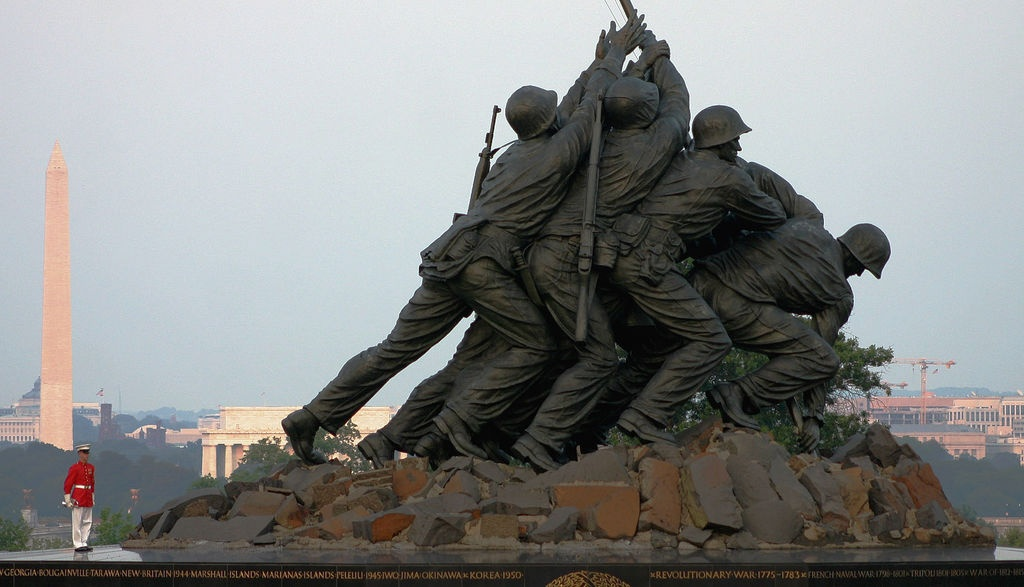
\includegraphics[width = 0.3\textwidth]{images/28979823.jpg}}
% \hspace{5mm}
\subfloat{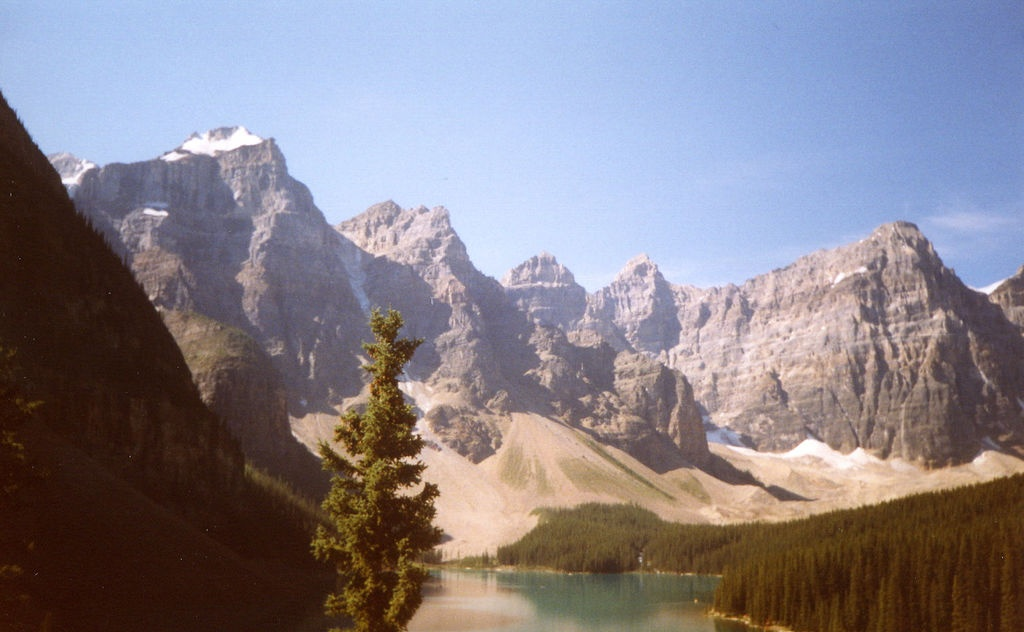
\includegraphics[width = 0.3\textwidth]{images/29018694.jpg}}
\hspace{5mm}
% \subfloat{\includegraphics[width = 0.3\textwidth]{images/other1.jpg}}
% \hspace{5mm}
\subfloat{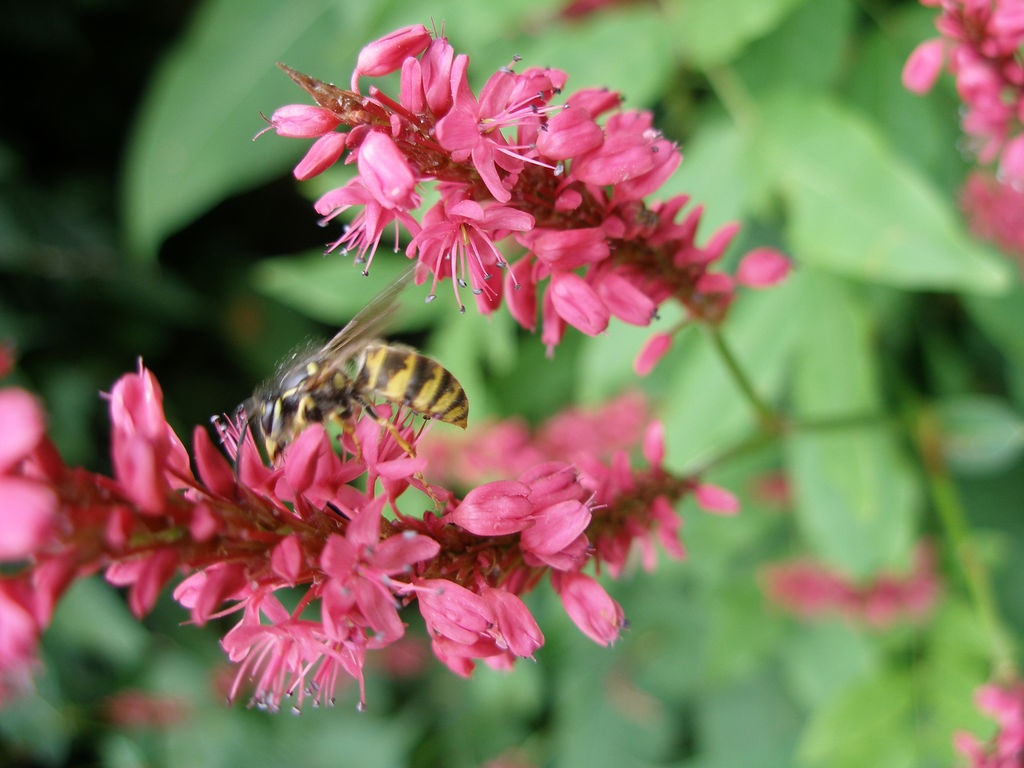
\includegraphics[width = 0.3\textwidth]{images/other2.jpg}}
\hspace{5mm}
\subfloat{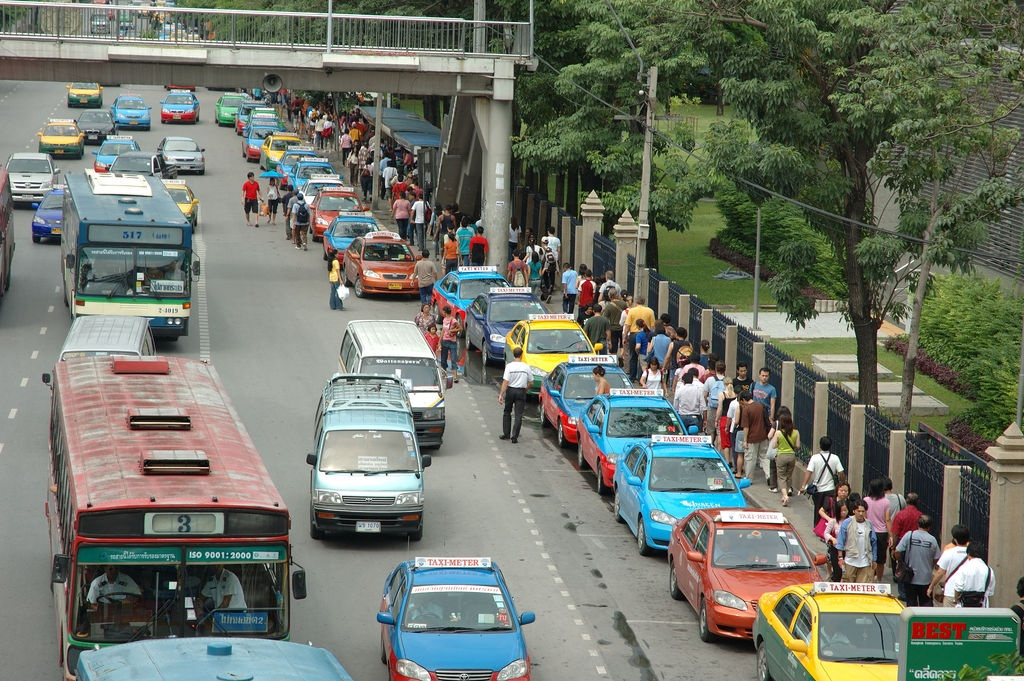
\includegraphics[width = 0.3\textwidth]{images/other3.jpg}}
\hspace{5mm}
\subfloat{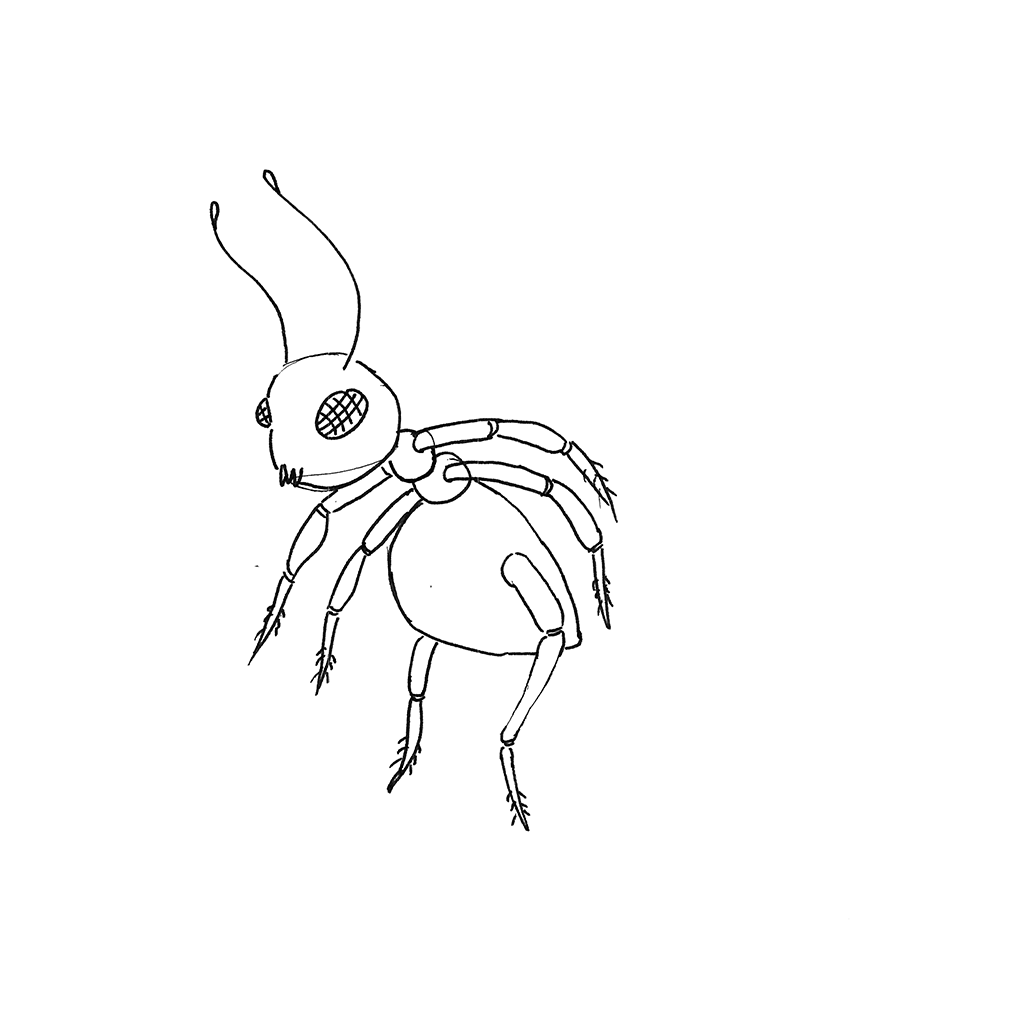
\includegraphics[width = 0.3\textwidth]{images/0.png}}
\hspace{5mm}
\subfloat{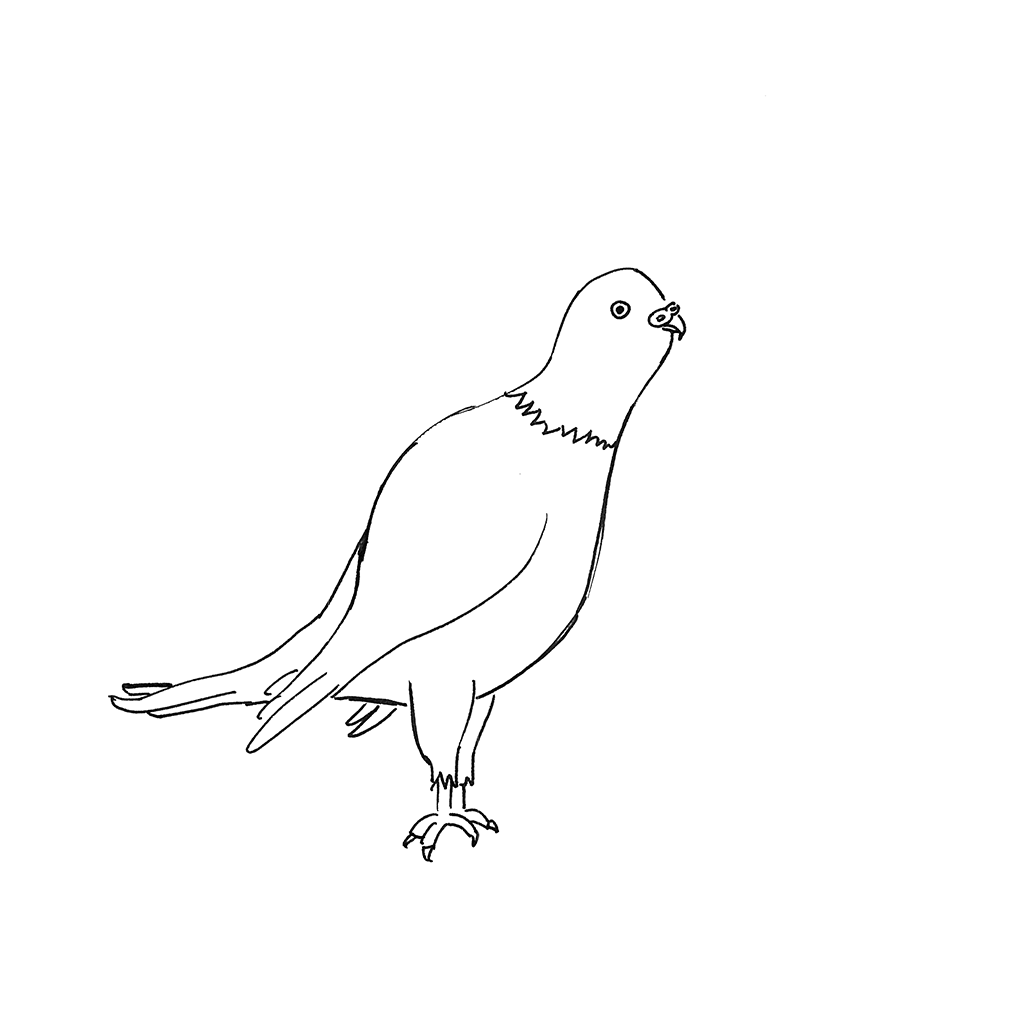
\includegraphics[width = 0.3\textwidth]{images/33.png}}
\hspace{5mm}
\subfloat{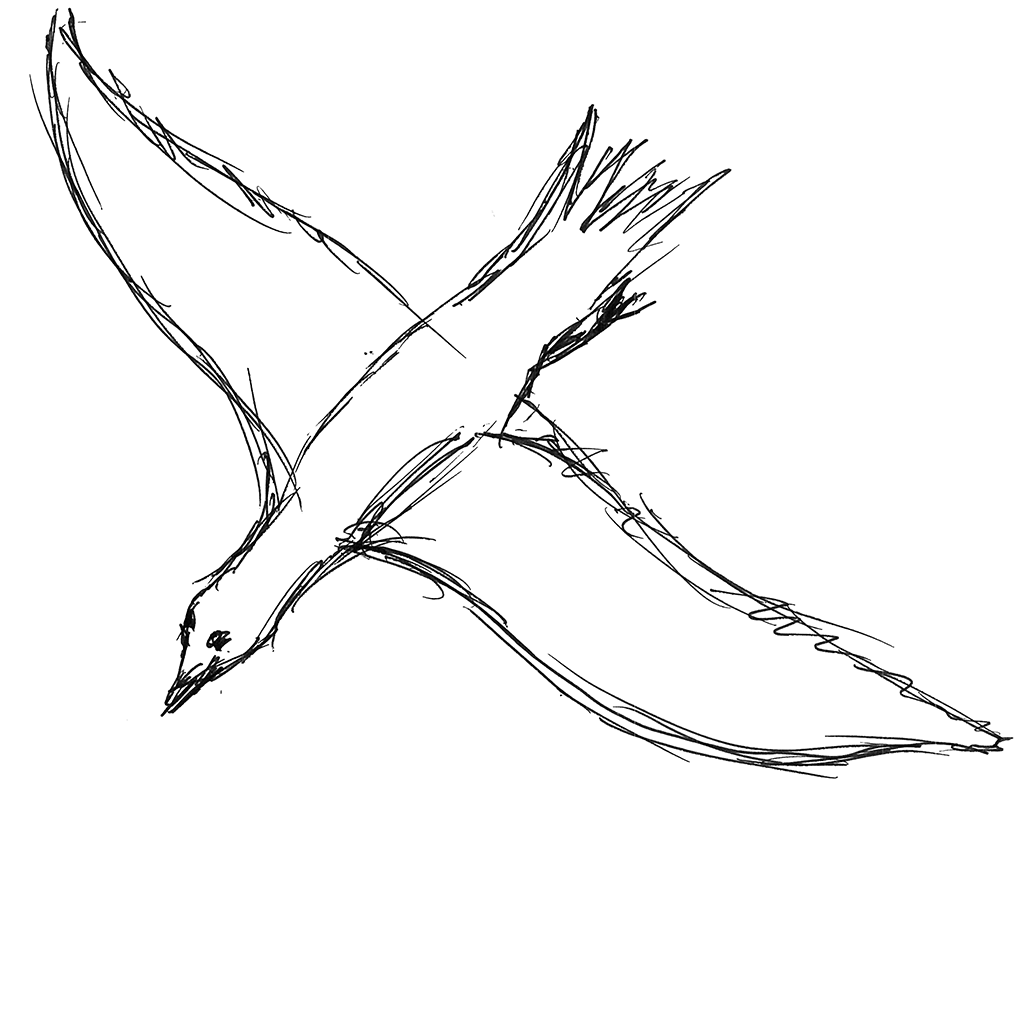
\includegraphics[width = 0.3\textwidth]{images/35.png}}
\hspace{5mm}
\caption{Example images of natural image and sketch training sets}
\label{fig:database_images}
\end{figure}

\section{Performance measurement}
Before we go further and present the experiments and results it is necessary to
introduce some additional terms. Such as metrics to measure their performance.

\paragraph{Mean squared error (MSE)}  An error measurement that
describes the error between a given or measured reference signal $\vec{x}$
and the reconstruction $\vec{\tilde{x}}$ of it. Mathematically it is defined as
the average of the squared error between two signals.
%The mean squared error is defined as:
\begin{equation*}
 MSE = \frac{1}{n} \sum_{i=0}^{n} \left( {\lVert x_i -
\tilde{x}_i\rVert^{2}}\right)
\end{equation*}
%We primarily use it for testing dictionary learning convergence and as a
%sub term for the measurement described in the next paragraph.

\paragraph{Peak signal-to-noise ratio (PSNR)} Describes the ratio between the
noise affecting a signal and the maximum possible signal amplitude. It is
expressed in a logarithmic decibel scale and undefined for zero
noise.
\begin{equation*}
 PSNR = 20 \cdot \log_{10} \left(\frac{MAX}{\sqrt{MSE}}\right)
\end{equation*}
Where $MAX$ is the maximum possible value of our signal. For an 8-bit
image it would be 255. For a 32-bit normalized image it would be 1.
% $MSE$ is the mean squared error between a reference signal and its
% reconstruction. 

The PSNR is primarily used for comparison of the reconstruction quality of
lossy compression algorithms. Typical values for a lossy reconstruction lie in
a range between 30dB and 
50dB.\footnote{\url{http://en.wikipedia.org/wiki/Peak_signal-to-noise_ratio}}
%e.g. relevant for de-noise

\paragraph{Bits per pixel (bpp)} 
For the comparison of compression ratios of images another well known practice
is to measure the required \emph{bits per pixel} short bpp. The bbp are
calculated by dividing size of the image data by the image's dimensions. For
example an uncompressed RGB color image with 8-bit color depth requires
$24bpp$, respectively a gray scale image with 8-bit for a single
channel requires $8bpp$. Compression algorithms are able to encode
multiple pixels with few coefficient leading to much lower bpp rates.
Looking at other well known compression algorithms such as JPEG or
JPEG 2000 a common ratio is about $\sim1.8bpp$ for average
quality compression (JPEG quality of 50) and less than $\sim1bpp$ for
lower compression.

%\Todo{optinal: example image?, lower bit rates, Lewicki estimate for sparse
%coding}

\paragraph{Test data}
In addition to the introduced metrics it is common practice to use some image
sets to compare test results of the different algorithms and parameter
configurations. As the dictionaries are specifically trained for
reconstruction of data in the training sets
(\prettyref{fig:database_images}). It is mandatory to also use
these images to test the reconstruction and compression quality. 

In addition to this we want to know how good the dictionaries can compress
images outside the database respectively the training set. For
those comparisons we use a selection (\prettyref{fig:USC-SIPI}) from a
well known set of standard test images from the \emph{USC-SIPI Image
Database}\footnote{\url{http://sipi.usc.edu/database/}}. 
%Including pictures such as Lena, Mandrill and Peppers.
\begin{figure}[H]
\centering
%\subfloat{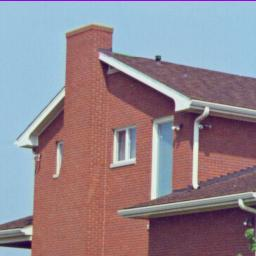
\includegraphics[width = 0.3\textwidth]{images/4_1_05.jpg}}
%\hspace{5mm}
\subfloat{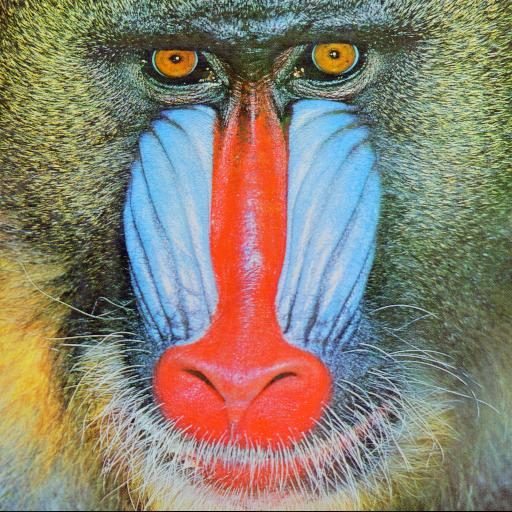
\includegraphics[width = 0.3\textwidth]{images/4_2_03.jpg}}
\hspace{5mm}
\subfloat{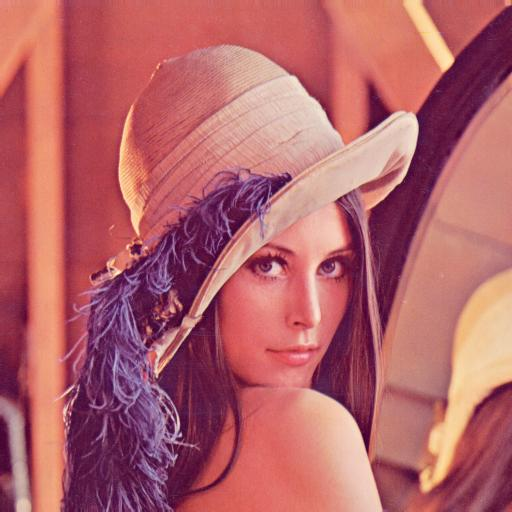
\includegraphics[width = 0.3\textwidth]{images/4_2_04.jpg}}
\hspace{5mm}
%\subfloat{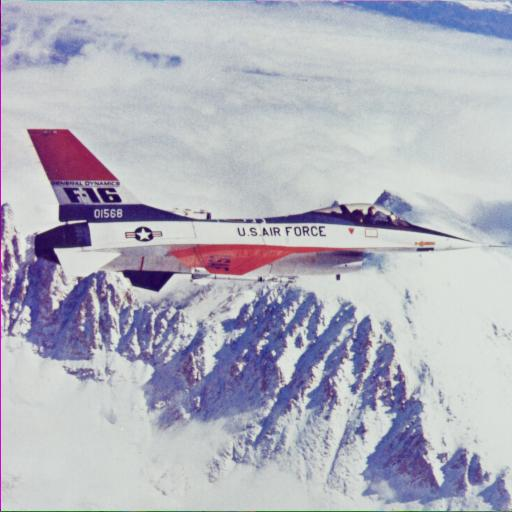
\includegraphics[width = 0.3\textwidth]{images/4_2_05.jpg}}
%\hspace{5mm}
%\subfloat{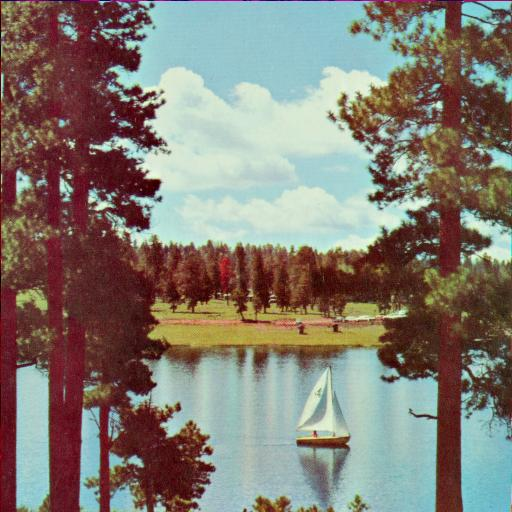
\includegraphics[width = 0.3\textwidth]{images/4_2_06.jpg}}
%\hspace{5mm}
\subfloat{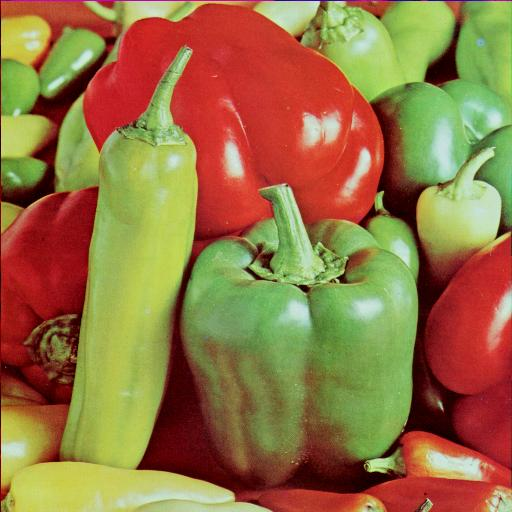
\includegraphics[width = 0.3\textwidth]{images/4_2_07.jpg}}
\caption{Example images from USC-SIPI Image Database}
\label{fig:USC-SIPI}
\end{figure}

\section{Hardware setup} 
Computations are made on a cluster consisting of 100 clients. Each 
configured with a AMD Athlon 64 X2 (2x2.6GHz) and 3GB RAM.
The operating system running is Debian Linux with 32-bit kernel. 

\section{Learning parameters}
At first we need to find start parameters for the dictionary learning
algorithm to experiment with large sets of different samples and big
dictionaries. This involves the average number of learning
coefficients, block size and sample selection strategy.

Mairal et al. already proposed some learning parameters for their online
learning algorithm. But like most others they only learn dictionaries with
a small redundancy of up to four and compact training sets with 100,000
to 1,000,000 samples that get randomly evaluated until convergence of the
dictionary.

We want to find start settings for experiments with large sets of
different samples with no re-evaluation of samples and dictionaries
with much bigger redundancy of 10 to 50.

% For the small training sets Mairal et al. suggest mini-batch sizes of two to
% four times the size of the the dictionary. No significant observations were
% made  and we stick to these sizes. 

\subsection{Number of learning coefficients}
An average of 10 learning coefficients is suggested as it produces enough
sparseness and leads to good and fast convergence of the dictionaries.
We test if this also applies to big numbers of samples and bigger
dictionaries. We compare the reconstruction quality depending on the average
number of coefficients in the learning process. 
%The following graphs show the avarage of a set of test images from the training
%set. 
Both OMP (\prettyref{fig:coeffsOMP}) and LARS-Lasso
(\prettyref{fig:coeffsLasso}) runs are made with the following
configuration.
\begin{table}[H]
%\caption{Configuration}
\centering
\begin{tabular}{| c | c | c |}
\hline
\hline
dict. size & block size & batch size \\
\hline
1024 & $8\times 8$ & 4000  \\
\hline
\end{tabular}
\end{table}
%\newpage
\begin{figure}[H]
\centering
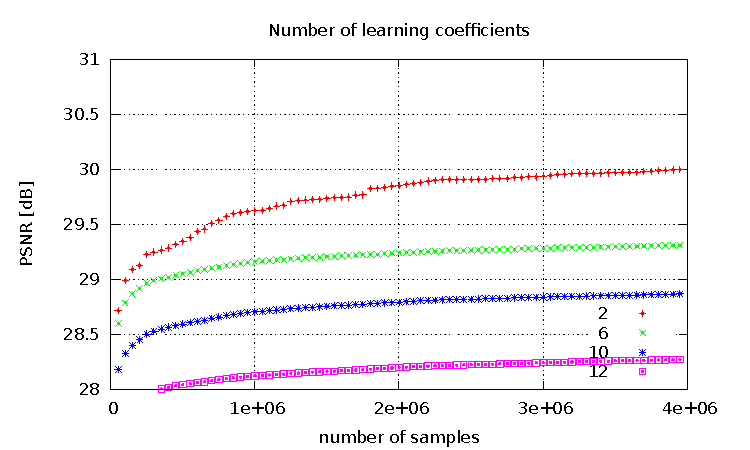
\includegraphics[width =
1.0\textwidth]{../tests/results/coeffsConvergOMP.pdf}
\caption{Reconstruction quality for different learning coefficients (OMP)}
\label{fig:coeffsOMP}
\end{figure}
\begin{figure}[H]
\centering
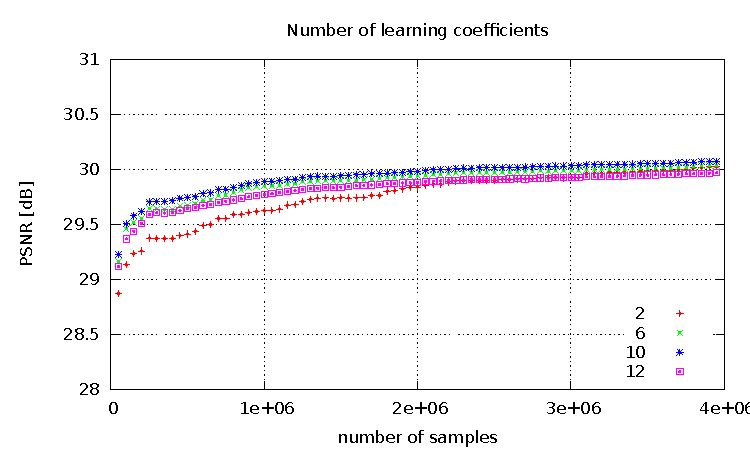
\includegraphics[width = 1.0\textwidth]{../tests/results/coeffsConverg.pdf}
\caption{Reconstruction quality for different learning coefficients (LARS)}
\label{fig:coeffsLasso}
\end{figure}
% \begin{figure}[H]
% \centering
% \subfloat[2]{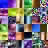
\includegraphics[width =
% 0.2\textwidth]{images/coeffsConvergOMP_0_1.jpg}}
% \hspace{15mm}
% \subfloat[10]{
\includegraphics[width =
% 0.2\textwidth]{images/coeffsConvergOMP_4_1.jpg}}
% \caption{after 50,000 samples}
% \label{fig:coeffsOMP50}
% \end{figure}
% \begin{figure}[H]
% \centering
% \subfloat[2]{
\includegraphics[width =
% 0.2\textwidth]{images/coeffsConvergOMP_0_2.jpg}}
% \hspace{15mm}
% \subfloat[10]{
\includegraphics[width =
% 0.2\textwidth]{images/coeffsConvergOMP_4_2.jpg}}
% \caption{after 2,000,000 samples}
% \label{fig:coeffsOMP2000}
% \end{figure}

% With high number of learning coefficents convergence is reached faster than
% with a low number of coefficents for OMP and LARS-Lasso.
% For larger training sets fewer coefficents can lead to better reconstruction
% quality. 
The first interesting observation is that both algorithms learn good
dictionaries with only a few coefficients. But while the LARS-Lasso is very
constant with different numbers of coefficients the quality of the OMP drops
with increasing number of coefficients. 

%\Todo{nach dict size verschieben?}
Unfortunately using only a few coefficients leads to problems with big
dictionaries. To illustrate this \prettyref{fig:dictSizeLassoBad} shows a
learning process of LARS-Lasso with about 4 learning coefficients.
\begin{figure}[h]
\centering
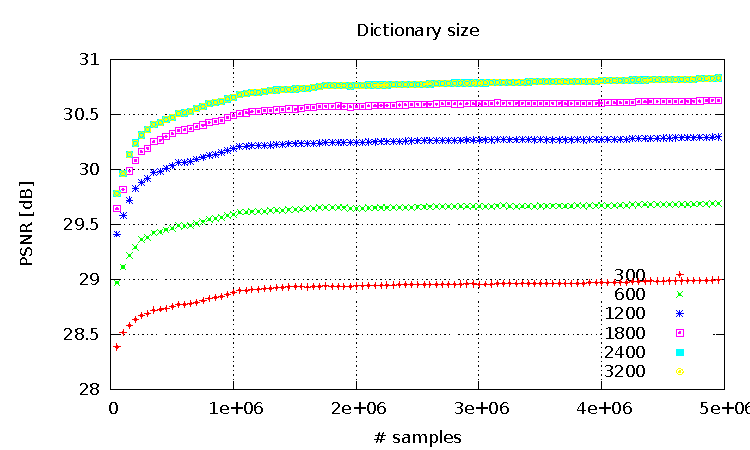
\includegraphics[width = 1.0\textwidth]{../tests/results/dictSizeLasso.pdf}
\caption[Reconstruction quality for different dictionary sizes
(LARS)]{Reconstruction quality for different dictionary sizes (LARS). 3,200 is
overlapping 2,400.}
\label{fig:dictSizeLassoBad}
\end{figure}
Notice two things in this graph. First convergence is almost reached
after 1,000,000 - 2,000,000 training samples. Second, even though the PSNR is a
logarithmic scale, increasing the dictionary size reaches a maximum at
about 2,400 atoms (3,200 is overlapping 2,400). 

The problem is that both algorithms do not learn enough atoms with too few
learning coefficients. Leaving a lot of the dictionary almost untouched. This
can be addressed by increasing the number of learning coefficients.

But renders OMP useless for learning larger dictionaries. Further learning
experiments concentrate on the LARS-Lasso with the suggested setting of 10
learning coefficients.


%\Todo{verschieben? zusammenhang nicht klar}
We also notice that the LARS-Lasso produces dictionaries with better
reconstruction quality than the OMP.

% \begin{figure}[H]
% \centering
% 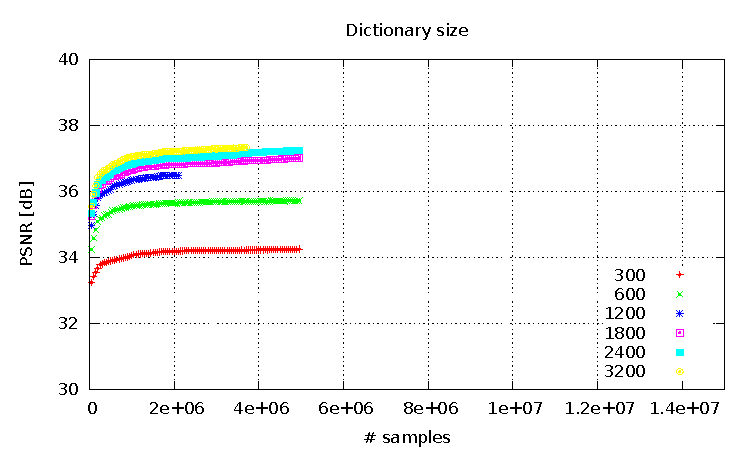
\includegraphics[width = 0.8\textwidth]{../tests/results/dictSizeOMP.pdf}
% \caption{reconstruction quality for different dictionary sizes (OMP)}
% \label{fig:dictSizeSizeOMPBad}
% \end{figure}


\newpage
\subsection{Block size}
After experiments on coefficients we compare the reconstruction quality
with different block sizes in the learning process for natural images. 

\prettyref{fig:blockSize} shows the results of dictionary
learning runs with block sizes of $8,...,20$. 
Each run a dictionary with redundancy of two. Coefficients for learning
and reconstruction are adjusted with an average of 2 coefficients for 16 pixels
of a block.

\begin{figure}[h]
\centering
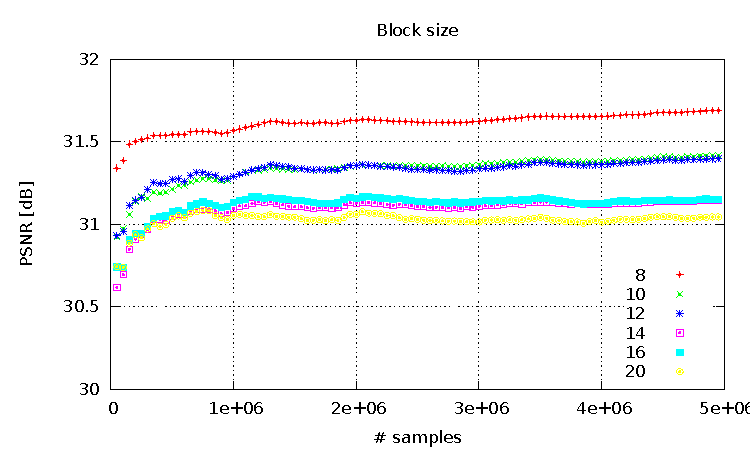
\includegraphics[width =
1.0\textwidth]{../tests/results/blockSizeConverg.pdf}
\caption{Reconstruction quality for different block sizes (LARS)}
\label{fig:blockSize}
\end{figure}

While the reconstruction quality decreases slightly with block size. 
The $8\times8$ block size has a significant better reconstruction quality. 
We start to understand why when we have a closer look at the structure of
the atoms. 

\newpage
\subsection{Structure of atoms}
%For the training set from natural JPEG images we tend to learn four major types
%of elements. 
From the traning set natural JPEG images the ODL algorithm learns atoms similar
to combinations of DCT atoms (\ref{fig:8atoms}a and  \ref{fig:8atoms}b) or
similar to wavelet atoms (\ref{fig:8atoms}c and \ref{fig:8atoms}d).

As our training sets consist of JPEG images it is likely that we actually learn
the block structure of JPEG images. This happens when extracting
$8\times 8$ block samples from JPEG images. \prettyref{fig:16jpeg_atoms}a shows
the effect when extracting $16\times 16$ blocks aligned to the JPEG block
structure.

When extracting overlapping samples with no alignment to the JPEG
blocks more wavelet like atoms show up for big block sizes
(\prettyref{fig:16jpeg_atoms}b) while the $8\times 8$ atoms do not change
significant. 

Having a closer Look at atoms learned from sketches we primarily see wavelet
like line segments (\prettyref{fig:sketch_atoms}) atoms.

Both dictionaries capture the structure the underlining signal provides. 
\begin{figure}[H]
\centering
\subfloat[]{
\includegraphics[width = 0.3\textwidth]{images/gradient.png}}
\hspace{5mm}
\subfloat[]{
\includegraphics[width = 0.3\textwidth]{images/checkerboard.png}}
\hspace{5mm}
\subfloat[]{
\includegraphics[width = 0.3\textwidth]{images/edges.png}}
\hspace{5mm}
\subfloat[]{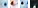
\includegraphics[width = 0.3\textwidth]{images/spot.png}}
\caption{$8\times 8$ atoms of natural images}
\label{fig:8atoms}
\end{figure}
\begin{figure}[H]
\centering
\subfloat[four $8\times 8$ micro
blocks]{
\includegraphics[width = 0.35\textwidth]{images/jpeg_atoms.png}}
\hspace{5mm}
\subfloat[$16\times 16$ atoms of natural images]{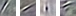
\includegraphics[width =
0.35\textwidth]{images/wavelet.png}}
\caption{$16\times 16$ atoms of natural images}
\label{fig:16jpeg_atoms}
\end{figure}
\begin{figure}[H]
\centering
\subfloat{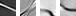
\includegraphics[width = 0.35\textwidth]{images/sketch_atoms.png}}
\caption{$16\times 16$ atoms of sketch images}
\label{fig:sketch_atoms}
\end{figure}



\clearpage

\section{Dictionary size}
With the right learning parameters to learn from large sets of
different images we want to know if reconstruction quality increases with
dictionaries size.

The following configuration is used for the experiments. 
\begin{table}[H]
\centering
\begin{tabular}{| c | c | c |}
\hline
%\multicolumn{3}{|c|}{configuration}\\
\hline
coefficients & block size & batch size \\
\hline
10 & $8\times 8$ & 4000  \\
\hline
\end{tabular}
\end{table}

\prettyref{fig:dictSizeGood} shows a different image than
\prettyref{fig:dictSizeLassoBad}. With the right learning parameters 
we better learn bigger dictionaries. We learned dictionaries with up to 8,000
elements and did not reach reconstruction maximum. But while quality increases
with size computational complexity increases too. We want to make the learning
step more independent of single machines. Being able to learn smaller parts of
big dictionaries or specific dictionaries.


\begin{figure}[h]
\centering
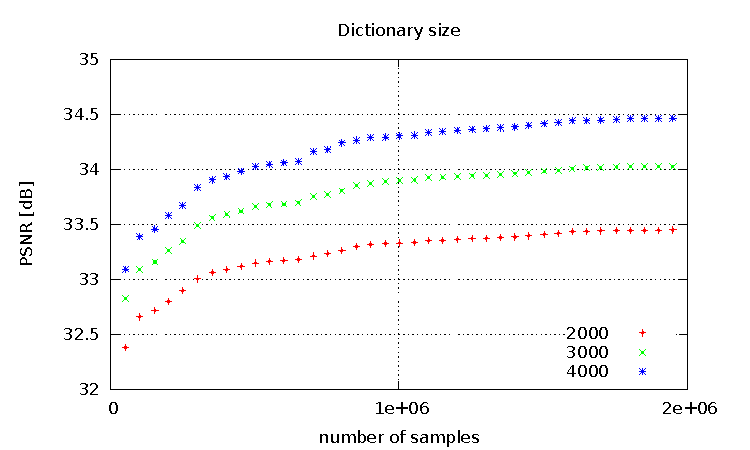
\includegraphics[width = 1.0\textwidth]{../tests/results/dictSizeLassoGod.pdf}
\caption{Reconstruction quality for different dictionary sizes (LARS)}
\label{fig:dictSizeGood}
\end{figure}

% We tried a diffrent strategy and addresed this issues with the clustering
% approach from \prettyref{sec:clustering}.
% \begin{figure}[h]
% \centering
% 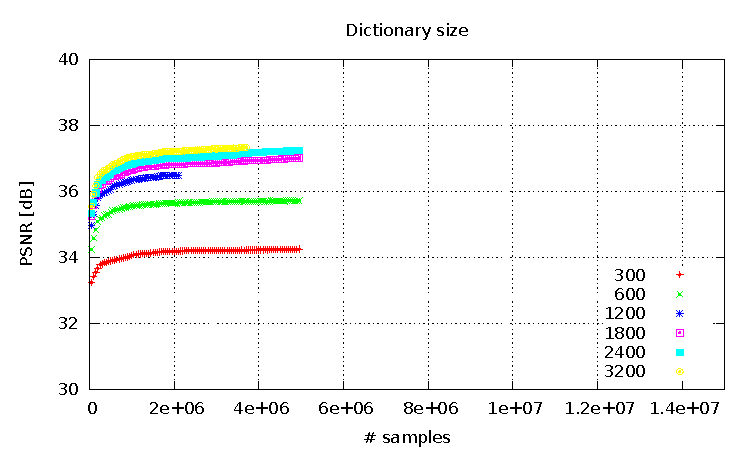
\includegraphics[width = 0.8\textwidth]{../tests/results/dictSizeOMP.pdf}
% \caption{reconstruction quality for different dictionary sizes (OMP)}
% \label{fig:dictSizeOMP}
% \end{figure}



\paragraph{Clustering}
We want to know if a dictionary merged from smaller dictionaries learned in a
cluster can lead to similar quality as a single big dictionary.

Learning with an average of 10 coefficients and a single dictionary of 4,000
elements are learned until convergence. And each of 10 clients in the cluster
learns a dictionary with 500 atoms from batches of 1,000 images. 

\prettyref{fig:coeffsConvergInc} shows reconstruction quality average for both
dictionaries.

We see that the merged dictionary can reconstruct images with equal quality
as the big dictionary. 


% \begin{table}[h]
% \centering
% \begin{tabular}{| l | c | c |}
% \hline\hline
% Images & single & merged \\
% \hline
% inside & $34,29172 \pm 3,61$ & $35,04152 \pm 3,48$  \\
% outside & $35.5104 \pm 0.0$ & $35.5104 \pm 0.0$ \\
% \hline
% \end{tabular}
% \caption{single vs. cluster}
% \end{table}

\begin{figure}[H]
\centering
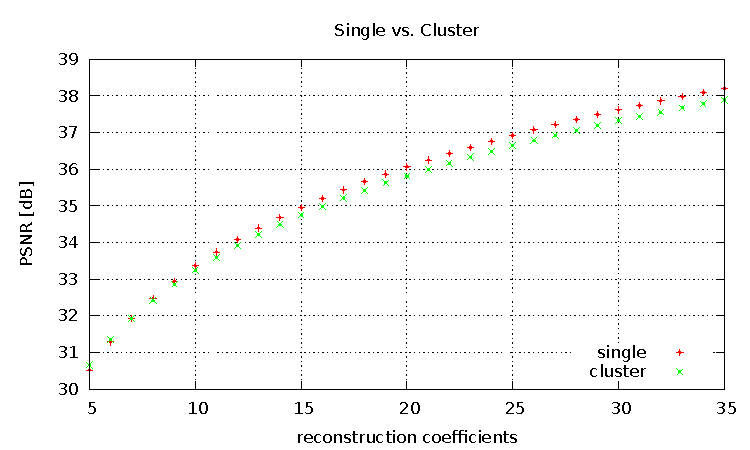
\includegraphics[width = 1.0\textwidth]{../tests/results/coeffsConvergInc.pdf}
\caption{Reconstruction quality of merged and single dictionary}
\label{fig:coeffsConvergInc}
\end{figure}


%And while machine limits prevent learning.
%Yet we want to see what we can already accomplish with the current
%dictionaries.

\clearpage
\section{Compression}
%Besides the ability of learned dictionaries 
We use the simple compression strategy from \prettyref{sec:compression}.
and compare it to a collection of JPEG and JPEG 2000 compressed images with the
same file size. Besides the raw pixel data, image formats usually contain a
certain amount of extra data from a file header and meta data. Fortunately we
can ignore this for simplification as the header data is only a few bytes and
large meta data was prevented during target compression. The selection of
images is limited by time consuming process of obtaining the right settings
for the sparse coding compression. 
%and not being actual pixel data. 
The objective is to investigate the compression quality of our algorithm and
the dictionary. 
% and if the extra amount of index data is a big hit on the overall load.

One benefit of the dictionary learning approach is the ability to learn and
use specific dictionaries for each group of images. We test this by learning a
dictionary from a set of sketch images and use it to compress sketches. A domain
in which the JPEG compression performs bad. As discovered before the natural
images like block sizes of $8\times 8$ this is not necessarily true for the
sketch images. They work fine with $16\times 16$ blocks and enable us to reduce
the amount of blocks.

The natural dictionary (\prettyref{fig:naturalDict}) consists of 4,000 $8 \times
8$ atoms merged from 100 sub dictionaries with 1,000 atoms. Each sub
dictionary was learned with 1,000 out of 100,000 images. Convergence of the
training process was already reached after 400 images. Taking less than 5
hours.

The sketch dictionary (\prettyref{fig:sketchDict}) consists of 1,000
$16\times 16$ atoms learned from roughtly 900 sketches.

\newpage
\begin{figure}[H]
\centering

\includegraphics[width = 0.66\textwidth]{images/natural_dict.jpg}
\caption{Natural dictionary for compression}\label{fig:naturalDict}
\end{figure}
\begin{figure}[H]
\centering

\includegraphics[width = 0.66\textwidth]{images/sketch_dict.jpg}
\caption{Sketch dictionary for compression}\label{fig:sketchDict}
\end{figure}


\clearpage
\subsection{Results}
This section presents the results of compression experiments with images
of \prettyref{fig:comp_images}. Compression coding was done with the OMP as it
turned out to work better with the quantization step of our algorithm and
requires less coefficients.

\begin{figure}[h]
\centering
\subfloat[]{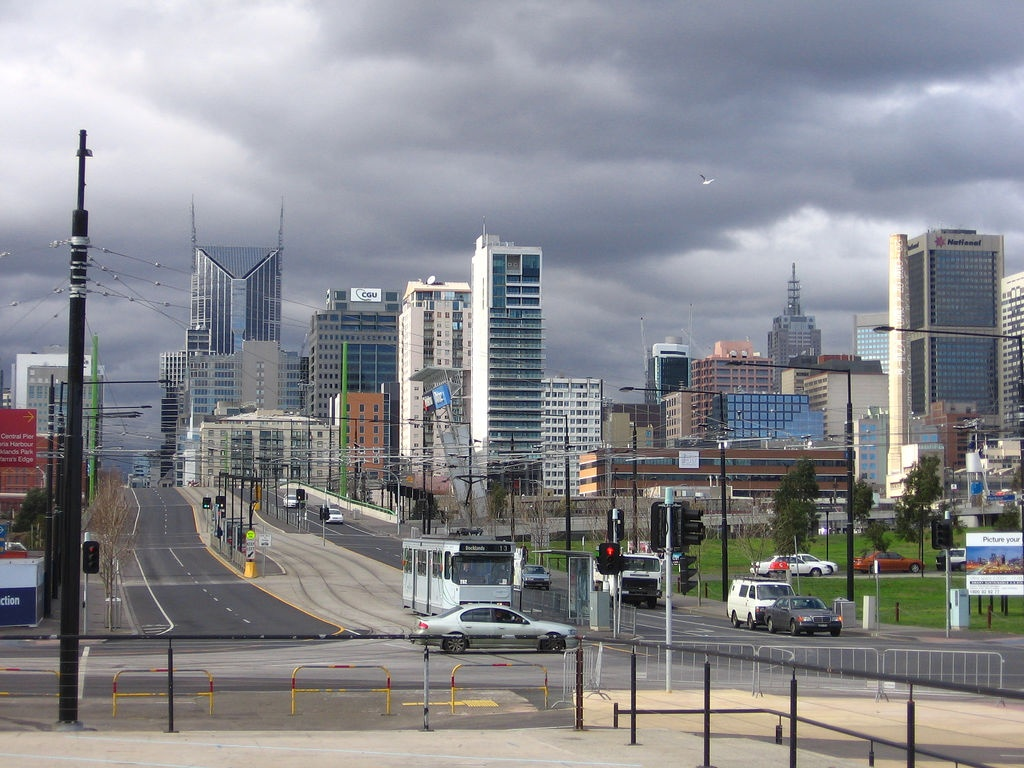
\includegraphics[width = 0.3\textwidth]{images/28952841.jpg}}
\hspace{5mm}
\subfloat[]{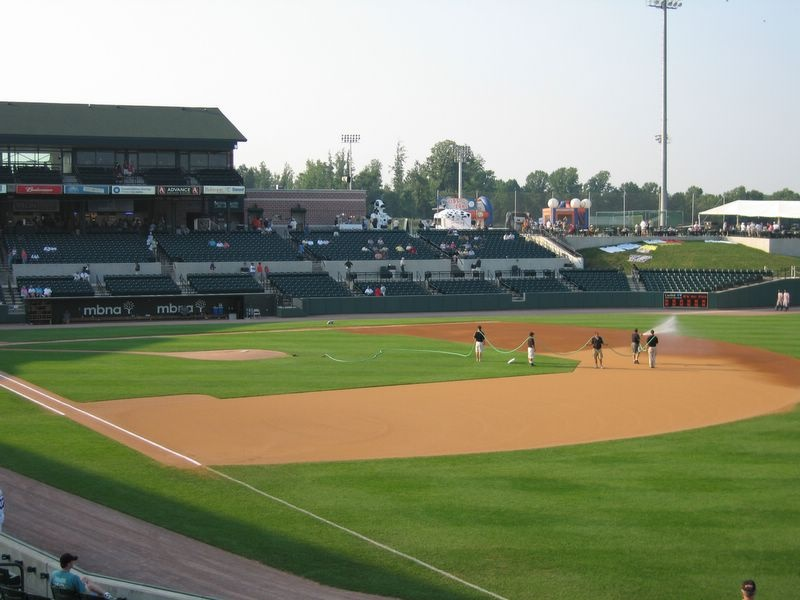
\includegraphics[width = 0.3\textwidth]{images/28894495.jpg}}
\hspace{5mm}
\subfloat[]{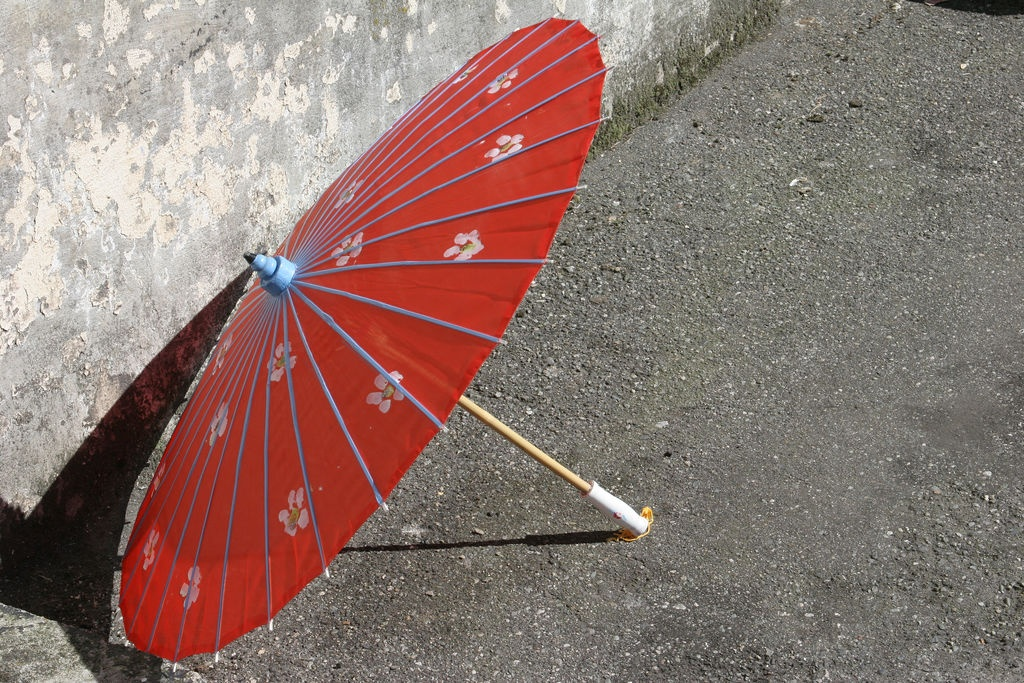
\includegraphics[width = 0.3\textwidth]{images/28874882.jpg}}
\hspace{5mm}
\subfloat[]{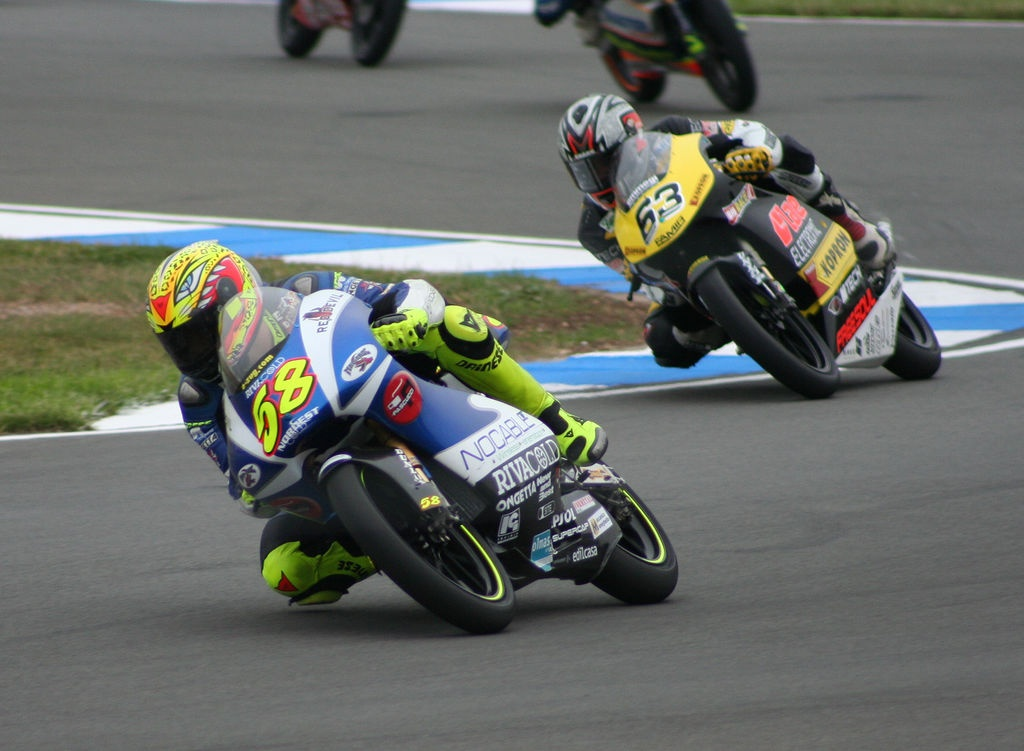
\includegraphics[width = 0.3\textwidth]{images/28803842.jpg}}
\hspace{5mm}
\subfloat[]{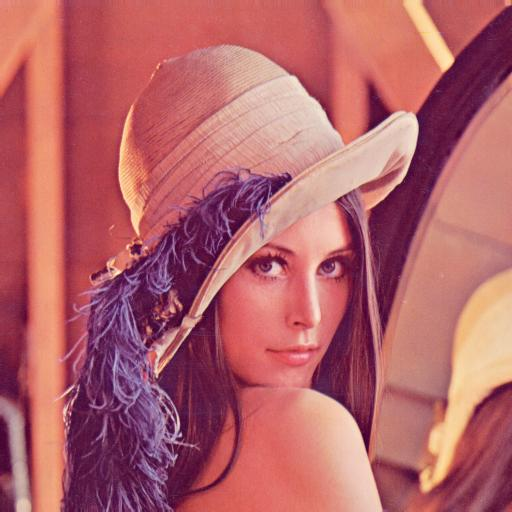
\includegraphics[width = 0.3\textwidth]{images/4_2_04.jpg}}
\hspace{5mm}
\subfloat[]{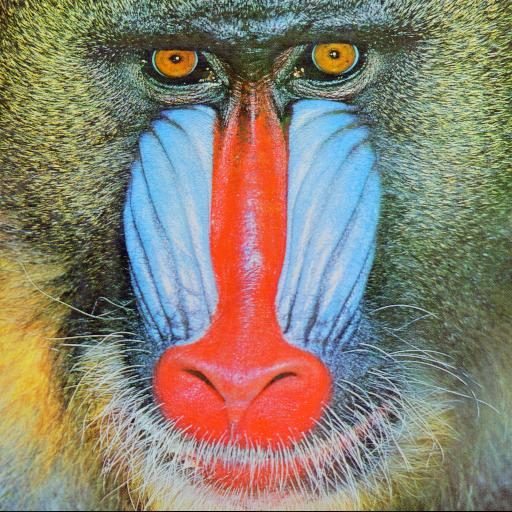
\includegraphics[width = 0.3\textwidth]{images/4_2_03.jpg}}
\hspace{5mm}
\subfloat[]{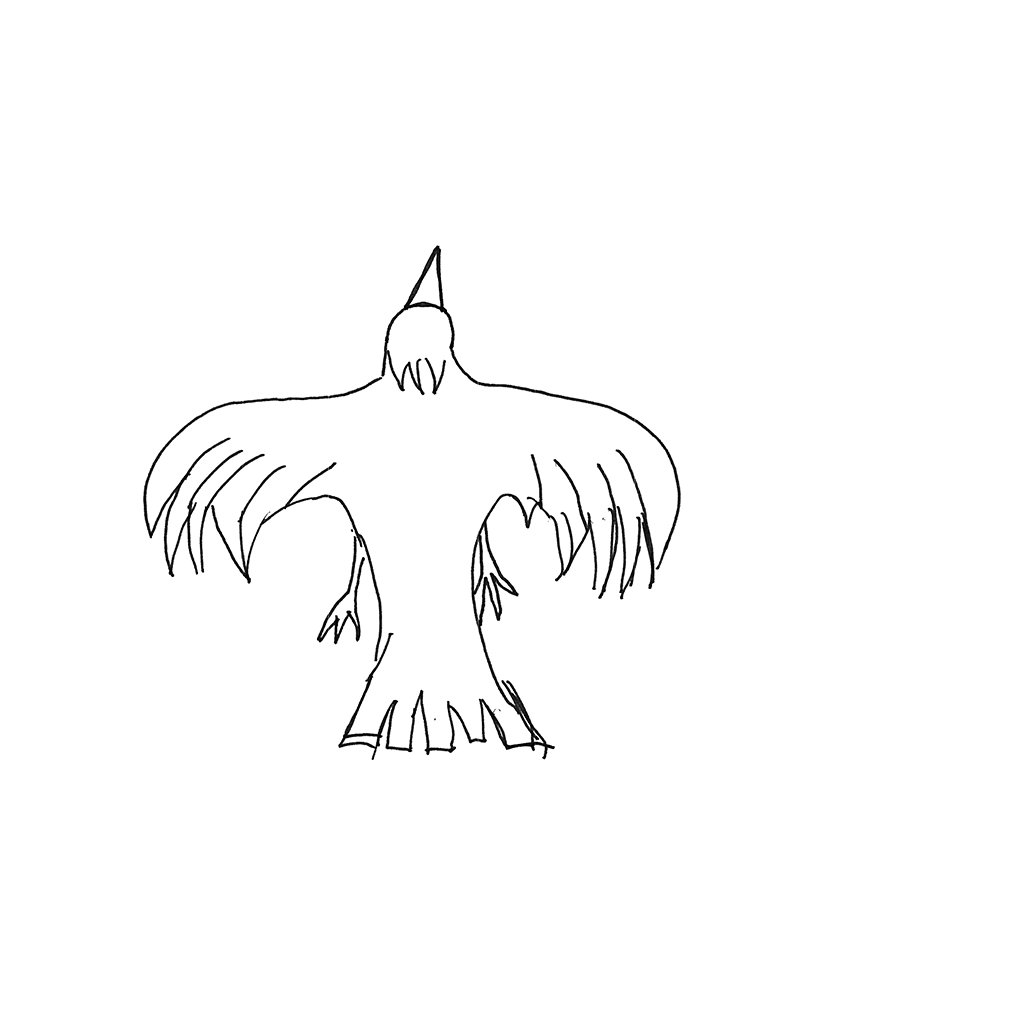
\includegraphics[width = 0.3\textwidth]{images/sketch1.jpg}}
\hspace{5mm}
\subfloat[]{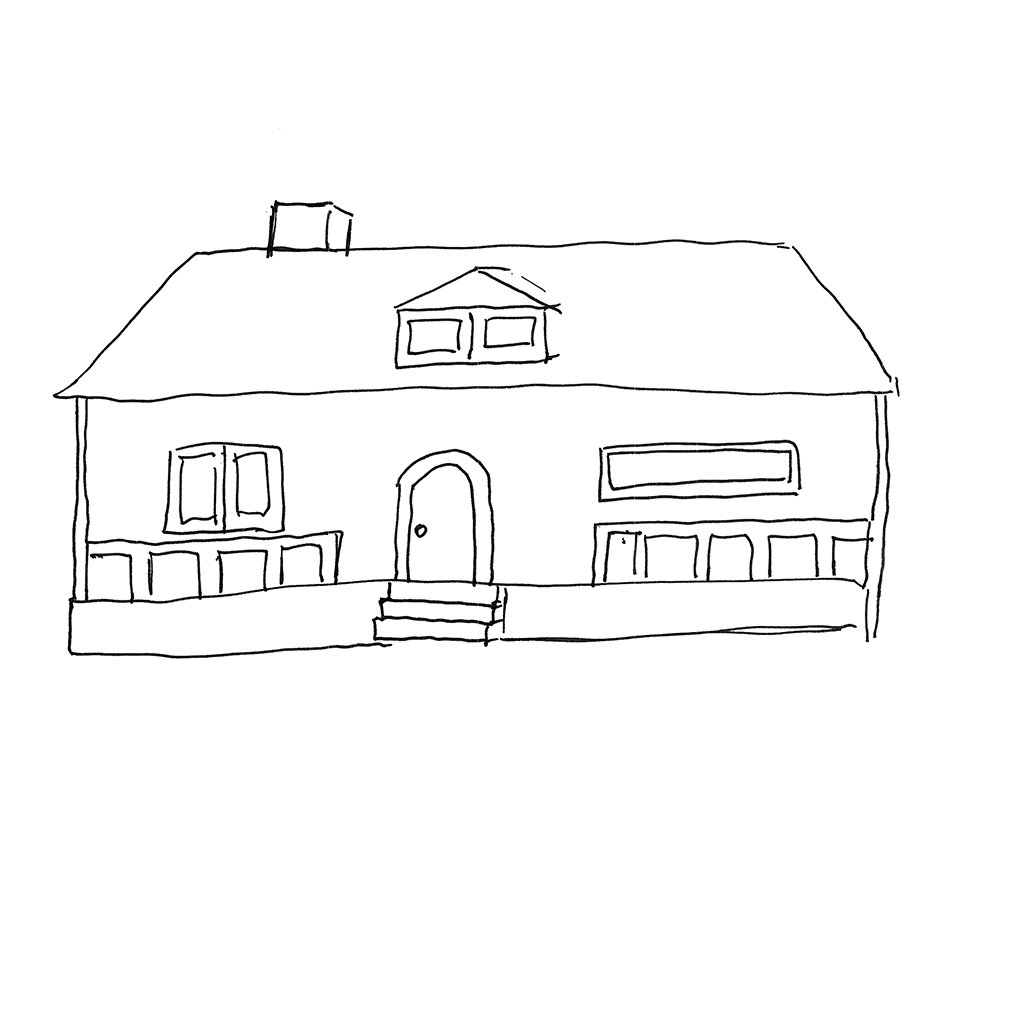
\includegraphics[width = 0.3\textwidth]{images/sketch2.jpg}}
\hspace{5mm}
\subfloat[]{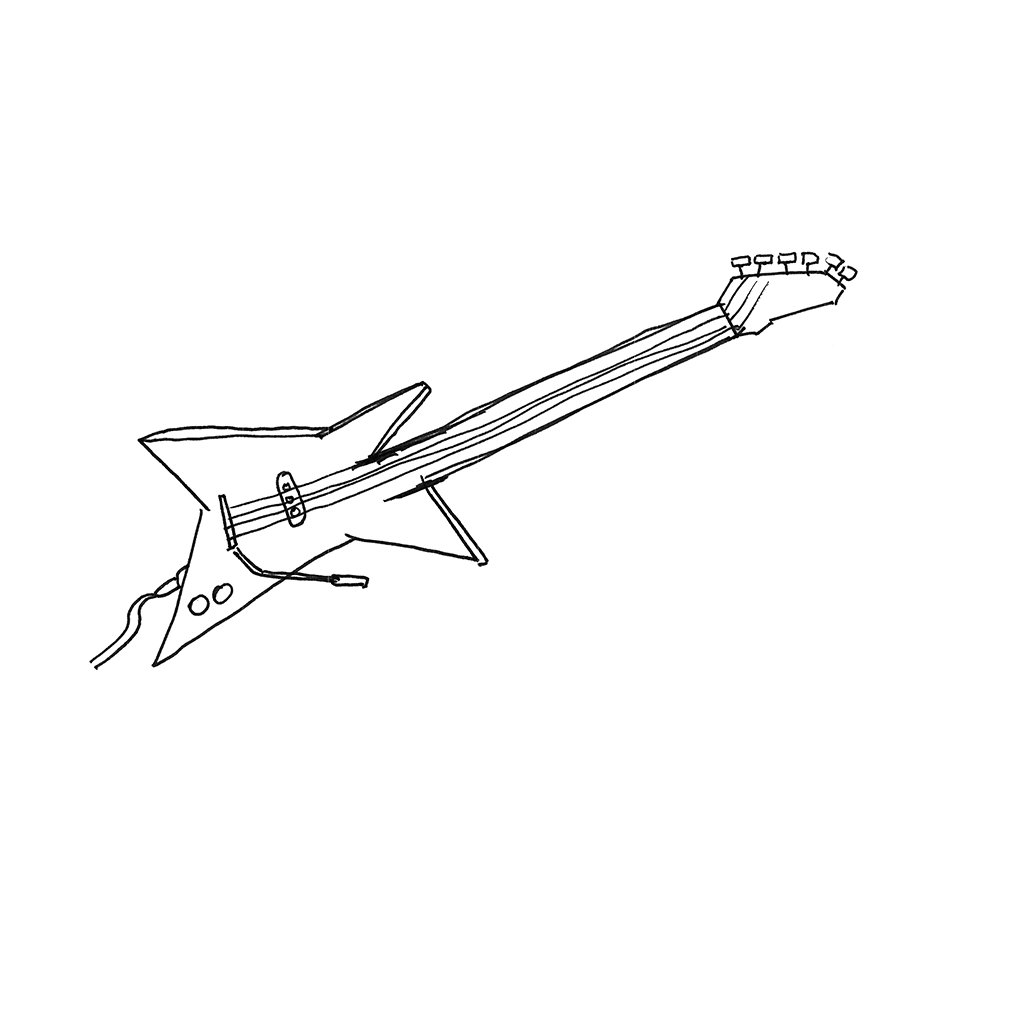
\includegraphics[width =
0.3\textwidth]{images/sketch3.jpg}\label{fig:sketch3}}
\hspace{5mm}
\caption{Images used for compression experiments}
\label{fig:comp_images}
\end{figure}

\newpage
\subsubsection{Natural images}
For the limited time available the results are promising.
Compression of the natural images achieves similar PSNR as the JPEG algorithm
(\prettyref{tab:compression1}) for high compression rates but does not reach the
JPEG 2000 quality.  Looking at a lower compression ratio the results are much
worse than JPEG or JPEG 2000 as the dictionaries have a limited maximum
reconstruction quality.

\begin{table}[h]
%\caption{single vs. cluster}
\centering

\begin{tabular}{| l l | c | c | c|}
\hline\hline
Image & bpp & SPRS & JPEG & JPEG2000 \\
\hline
\ref{fig:comp_images}a & 1.12 & 31.2205 & 32.3289 & 36.6103 \\
%a & 1.12 & 31.2205 & 42.7488 &  \\
\hline
\ref{fig:comp_images}b & 1.01 & 34.7735 & 35.0671 & 40.3299 \\
%b & 1.01 & 34.7735 & 49.4725 & \\
\hline
\ref{fig:comp_images}c & 1.8  & 29.0597 & 27.2556 & 31.7412 \\
%c & 1.8  & 34.5818 & 40.8959 &  \\
\hline
\ref{fig:comp_images}d & 0.74 & 35.0531 & 35.5104 & 39.4195 \\
%d & 1.47  & 35.9499 & 42.3517 &  \\
\hline
\ref{fig:comp_images}e & 0.66 & 28.2658 & 32.0171 & 32.7864 \\
\hline
\ref{fig:comp_images}f & 1.53 & 24.6843  & 24.8492 & 26.2794 \\
\hline
\end{tabular}
\caption{PSNR of compressed natural images}
\label{tab:compression1}.
\end{table} 

% \begin{figure}[h]
% \centering
% % \subfloat{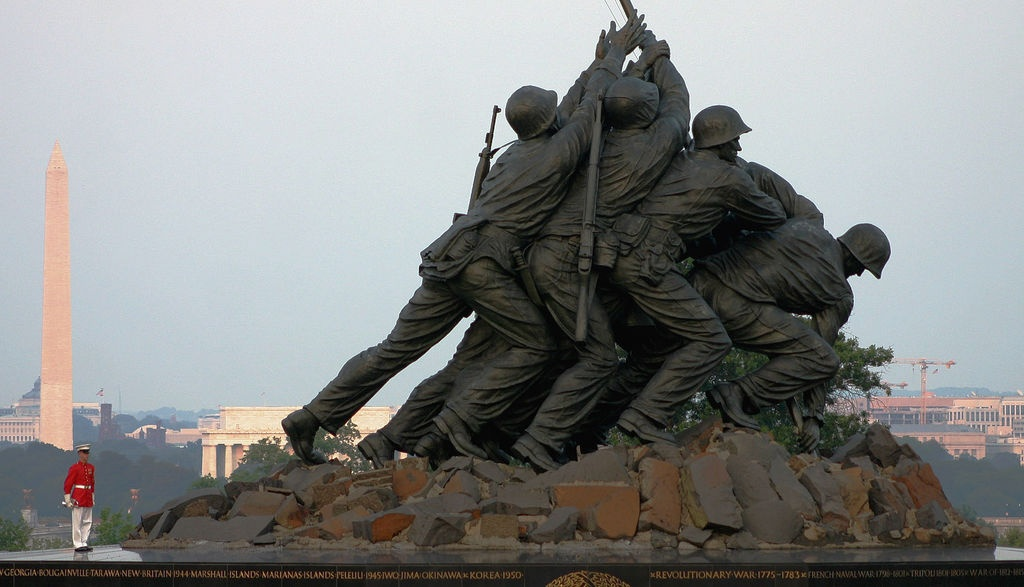
\includegraphics[width = 0.3\textwidth]{images/28979823.jpg}}
% % \hspace{5mm}
% % \subfloat{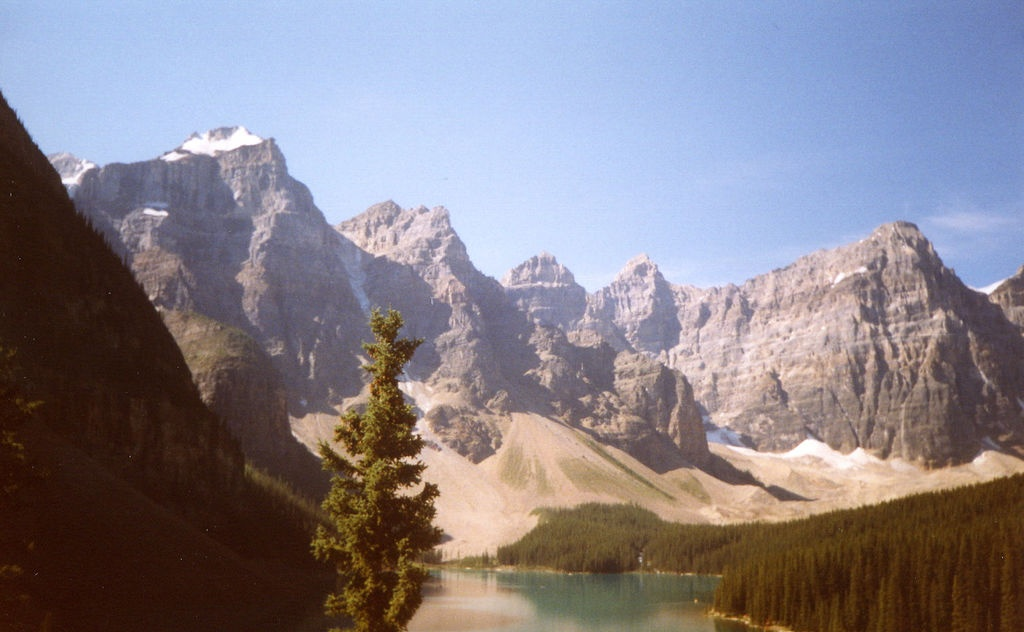
\includegraphics[width = 0.3\textwidth]{images/29018694.jpg}}
% % \hspace{5mm}
% \subfloat{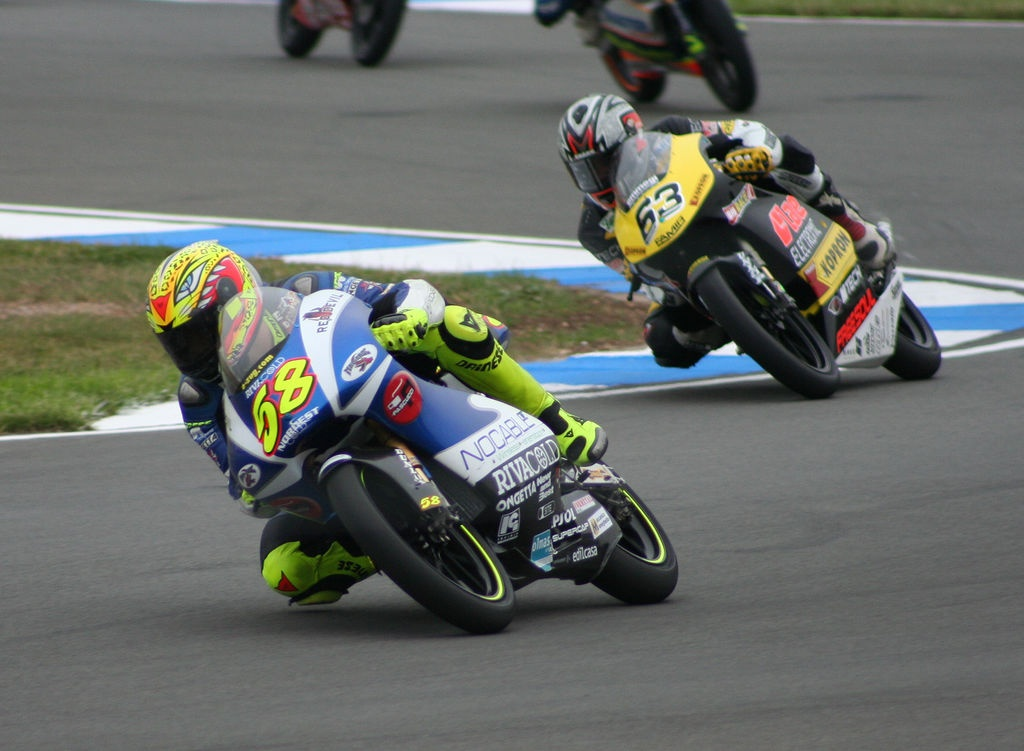
\includegraphics[width = 0.3\textwidth]{images/28803842.jpg}}
% \hspace{5mm}
% \subfloat{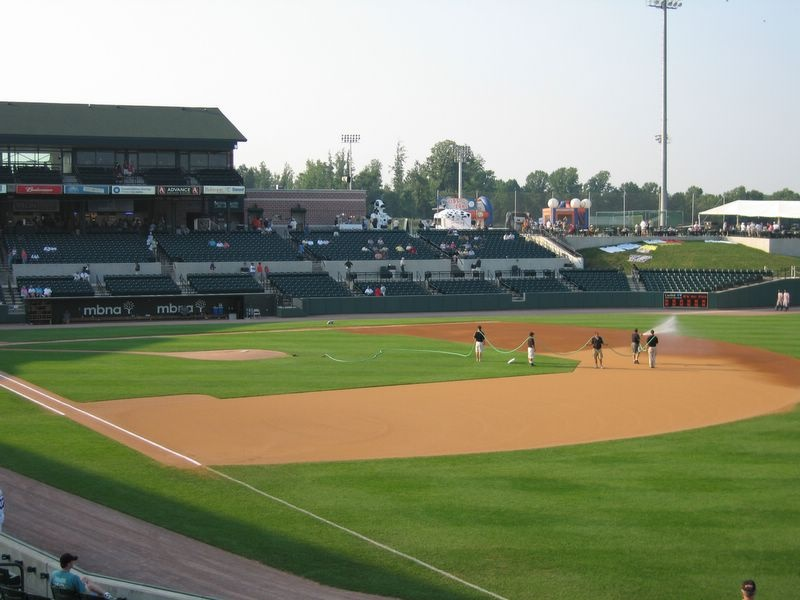
\includegraphics[width = 0.3\textwidth]{images/28894495.jpg}}
% \hspace{5mm}
% \subfloat{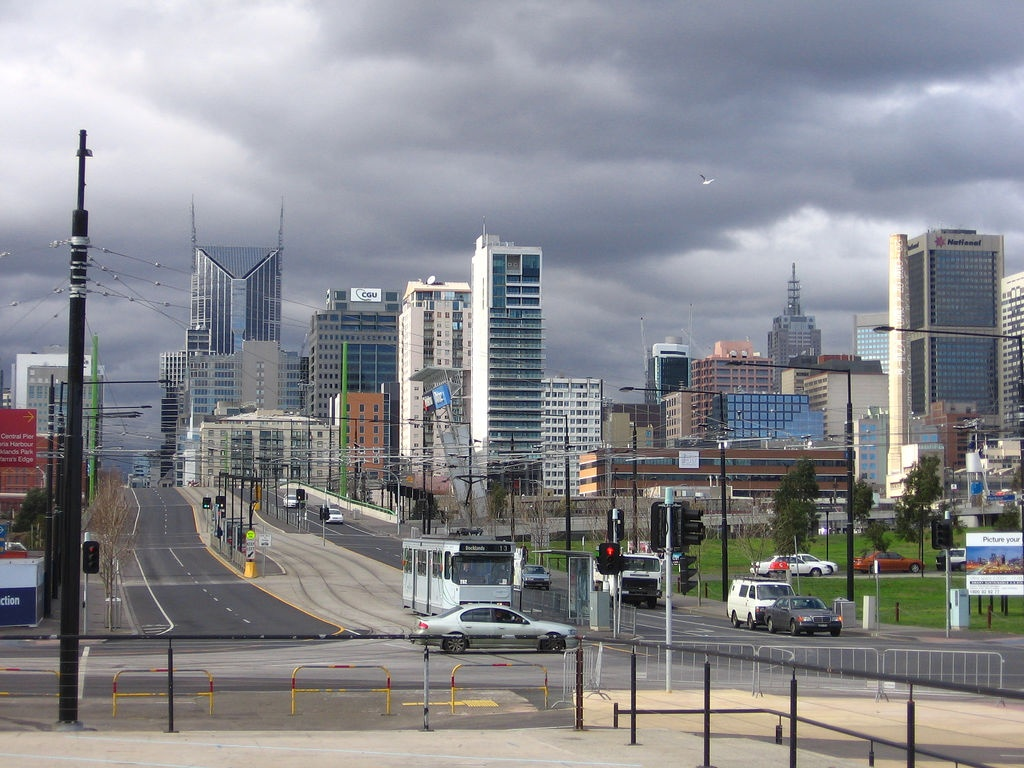
\includegraphics[width = 0.3\textwidth]{images/28952841.jpg}}
% \hspace{5mm}
% \subfloat{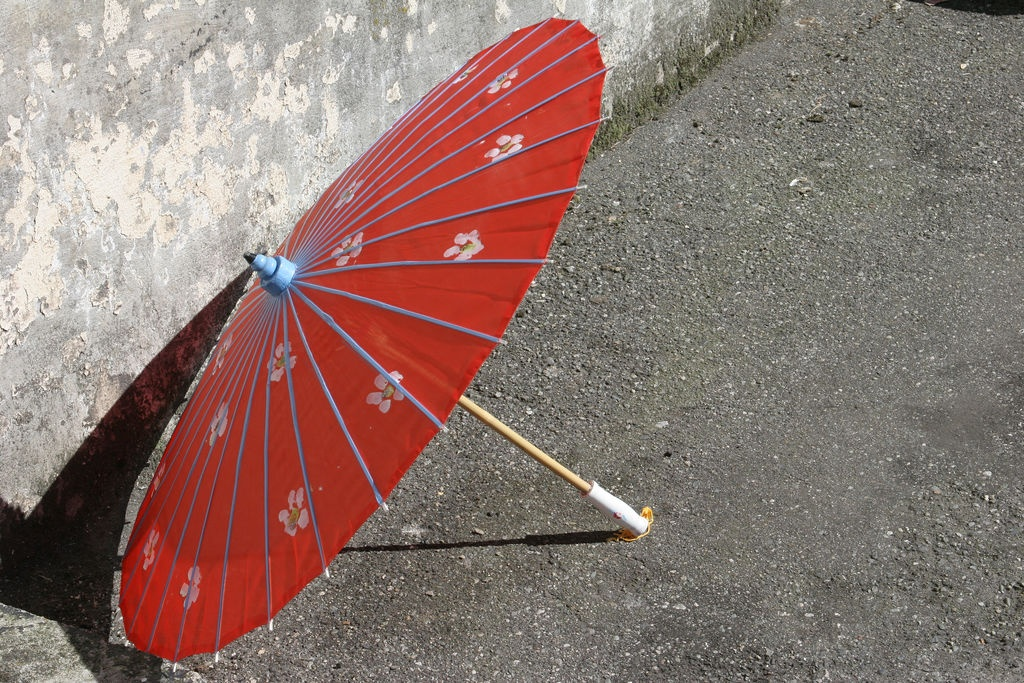
\includegraphics[width = 0.3\textwidth]{images/28874882.jpg}}
% \caption{natural images}
% %\label{fig:database_images}
% \end{figure}

\subsubsection{Sketches}
The high compression ratio results get even better when looking at the sketch
images. Our algorithm can surpass JPEG compression
(\prettyref{tab:compression2}) for low bits-per-pixel.
\prettyref{fig:magnified} shows a magnified segment of image
\ref{fig:sketch3} to illustrate the reconstruction features. Notice less
artifacts than in the JPEG images.

%The line segment atoms from the dictionary show similarities to the wavelet
%based JPEG 2000 compression.


\begin{table}[H]
%\caption{single vs. cluster}
\centering
\begin{tabular}{| c l | c | c | c|}
\hline\hline
Image & bpp & SPRS & JPEG & JPEG2000 \\
\hline
\ref{fig:comp_images}g & 0.084 & 33.9594 & 28.9578 & 38.3258  \\
%a & 0.084 & 33.9594 & 28.9578 & 38.3258  \\
\hline
\ref{fig:comp_images}h & 0.13 & 32.9002 & 34.5546 &  40.0159 \\
%b & 0.13 & 32.9002 & 34.5546 &  40.0159 \\
\hline
\ref{fig:comp_images}i & 0.08 & 32.5131 & 28.6558 & 36.3093  \\
%c & 0.08 & 32.5131 & 28.6558 & 36.3093  \\
\hline
\end{tabular}
\caption{PSNR of compressed sketch images}
\label{tab:compression2}
\end{table}
% \begin{figure}[h]
% \centering
% \setcounter{subfigure}{0}
% \subfloat[]{\includegraphics[width = 0.3\textwidth]{images/sketch1.jpg}}
% \hspace{5mm}
% \subfloat[]{\includegraphics[width = 0.3\textwidth]{images/sketch2.jpg}}
% \hspace{5mm}
% \subfloat[]{\includegraphics[width =
% 0.3\textwidth]{images/sketch3.jpg}\label{fig:sketch3}}
% \hspace{5mm}
% \caption{sketches}
% \label{fig:sketches}
% \end{figure}
%\newpage
\begin{figure}[h]
\centering
\subfloat[original]{\includegraphics[width =
0.40\textwidth]{images/sketch_png_1.png}}
\hspace{5mm}
\subfloat[SPRS]{\includegraphics[width =
0.40\textwidth]{images/sketch_sprs_1.png}}
\hspace{25mm}
\subfloat[JPEG]{\includegraphics[width =
0.40\textwidth]{images/sketch_jpeg_1.png}}
\hspace{5mm}
\subfloat[JPEG2000]{\includegraphics[width =
0.40\textwidth]{images/sketch_2000_1.png}}
\caption{Magnified segment of image \ref{fig:sketch3}}
\label{fig:magnified}
\end{figure}




















